\cite{clean-arch-book} mostra a Arquitetura Limpa, uma abordagem que tem por objetivo delimitar responsabilidades para cada um dos componentes em um software.
Esta abordagem produz softwares independentes de \emph{frameworks}, intefaces de usuário, bancos de dados e de qualquer agente externo, de modo que as regras de negócio sejam plenamente testáveis.

A Arquitetura Limpa divide as responsabilidades em quatro níveis: entidades, casos de uso, adaptadores de interfaces e agentes externos.
As entidades encapsulam regras de negócio inerentes ao domínio da aplicação.
Uma entidade pode ser um objeto com métodos, ou um conjunto de estruturas de dados e funções.

Os casos de uso encapsulam as regras específicas para o funcionamento da aplicação.
Eles fazem uso das regras de negócio presentes nas entidades para atingir os seus objetivos.
Não é esperado que mudanças em agentes externos impactem nos casos de uso.

Os adaptadores de interface são componentes responsáveis por converter dados de um formato para outro.
Eles são utilizados, por exemplo, para converter os dados de entidades para um banco de dados ou interface de usuário, e vice-versa.

A camada de agentes extenos é composta por \emph{frameworks}, bibliotecas de terceiros, bancos de dados e qualquer outro componente externo que auxilie na execução das regras de negócio.

A Figura~\ref{fig:clean_arch_circles} ilustra a Arquitetura Limpa como círculos concêntricos, onde cada círculo representa uma camada.
As camadas mais internas não interagem diretamente com as camadas mais externas.
São utilizadas abstrações para permitir que as camadas se comuniquem, respeitando assim o Princípio de Inversão de Dependências.

\begin{figure}[ht]
	\centering
	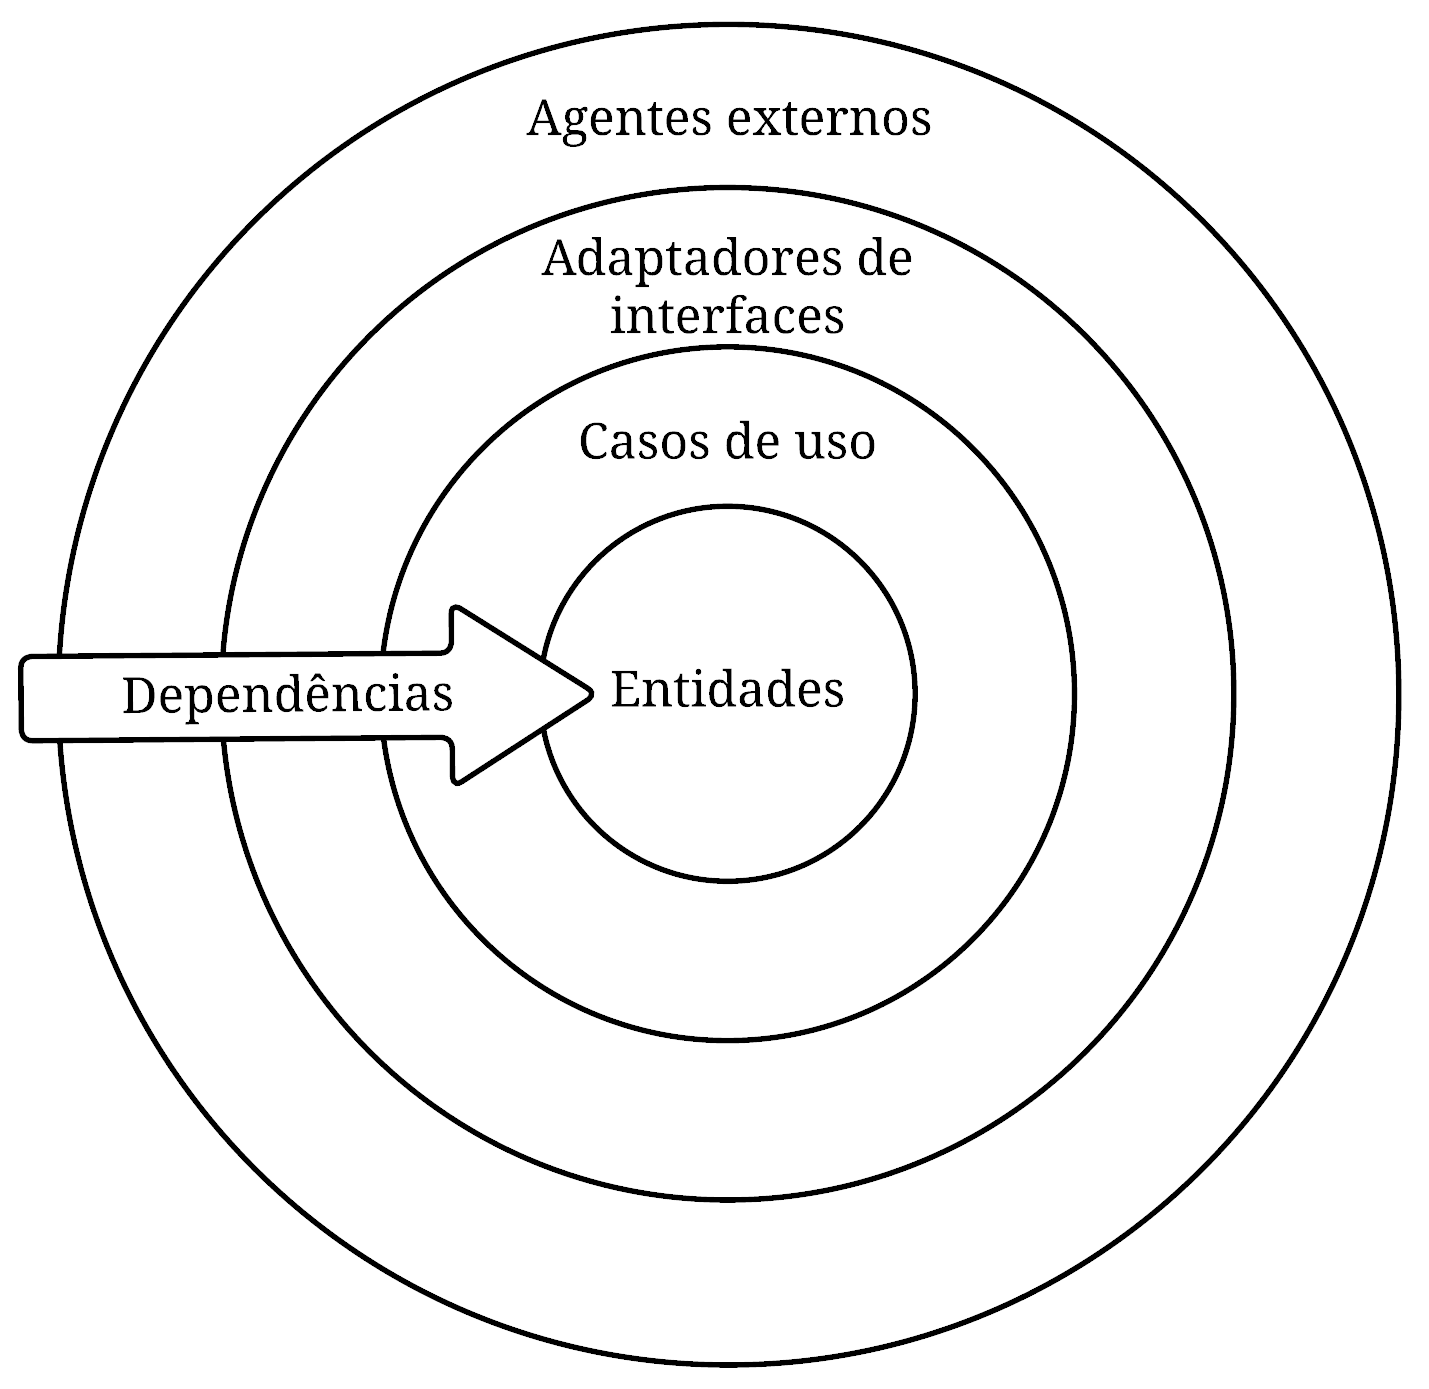
\includegraphics[width=0.52\textwidth]{images/clean_arch_circles.png}
	\caption{Camadas da Arquitetura Limpa e suas dependências}
	\label{fig:clean_arch_circles}
\end{figure}